\section{Durchführung} \label{sec:durchführung}

\subsection{Aufbau}

    Die Messung der Wärmeleitfähigkeit wird mithilfe einer Platte,
    auf der Stäbe aus Aluminium, Edelstahl und zwei verschieden breite Messing-Stäbe befestigt sind.
    Ein Peltierelement in der Mitte der Platte heizt oder kühlt die Stäbe.
    Für diese Einstellung ist ein Schalter mit den Optionen \enquote{\textbf{HEAT}} und \enquote{\textbf{COOL}} angebracht.
    An die Platte ist eine Spannung $U_\text{P}$ angeschlossen, sodass das Peltierelement mit maximalem
    Strom versorgt wird.

    \begin{figure}[H]
       \centering
       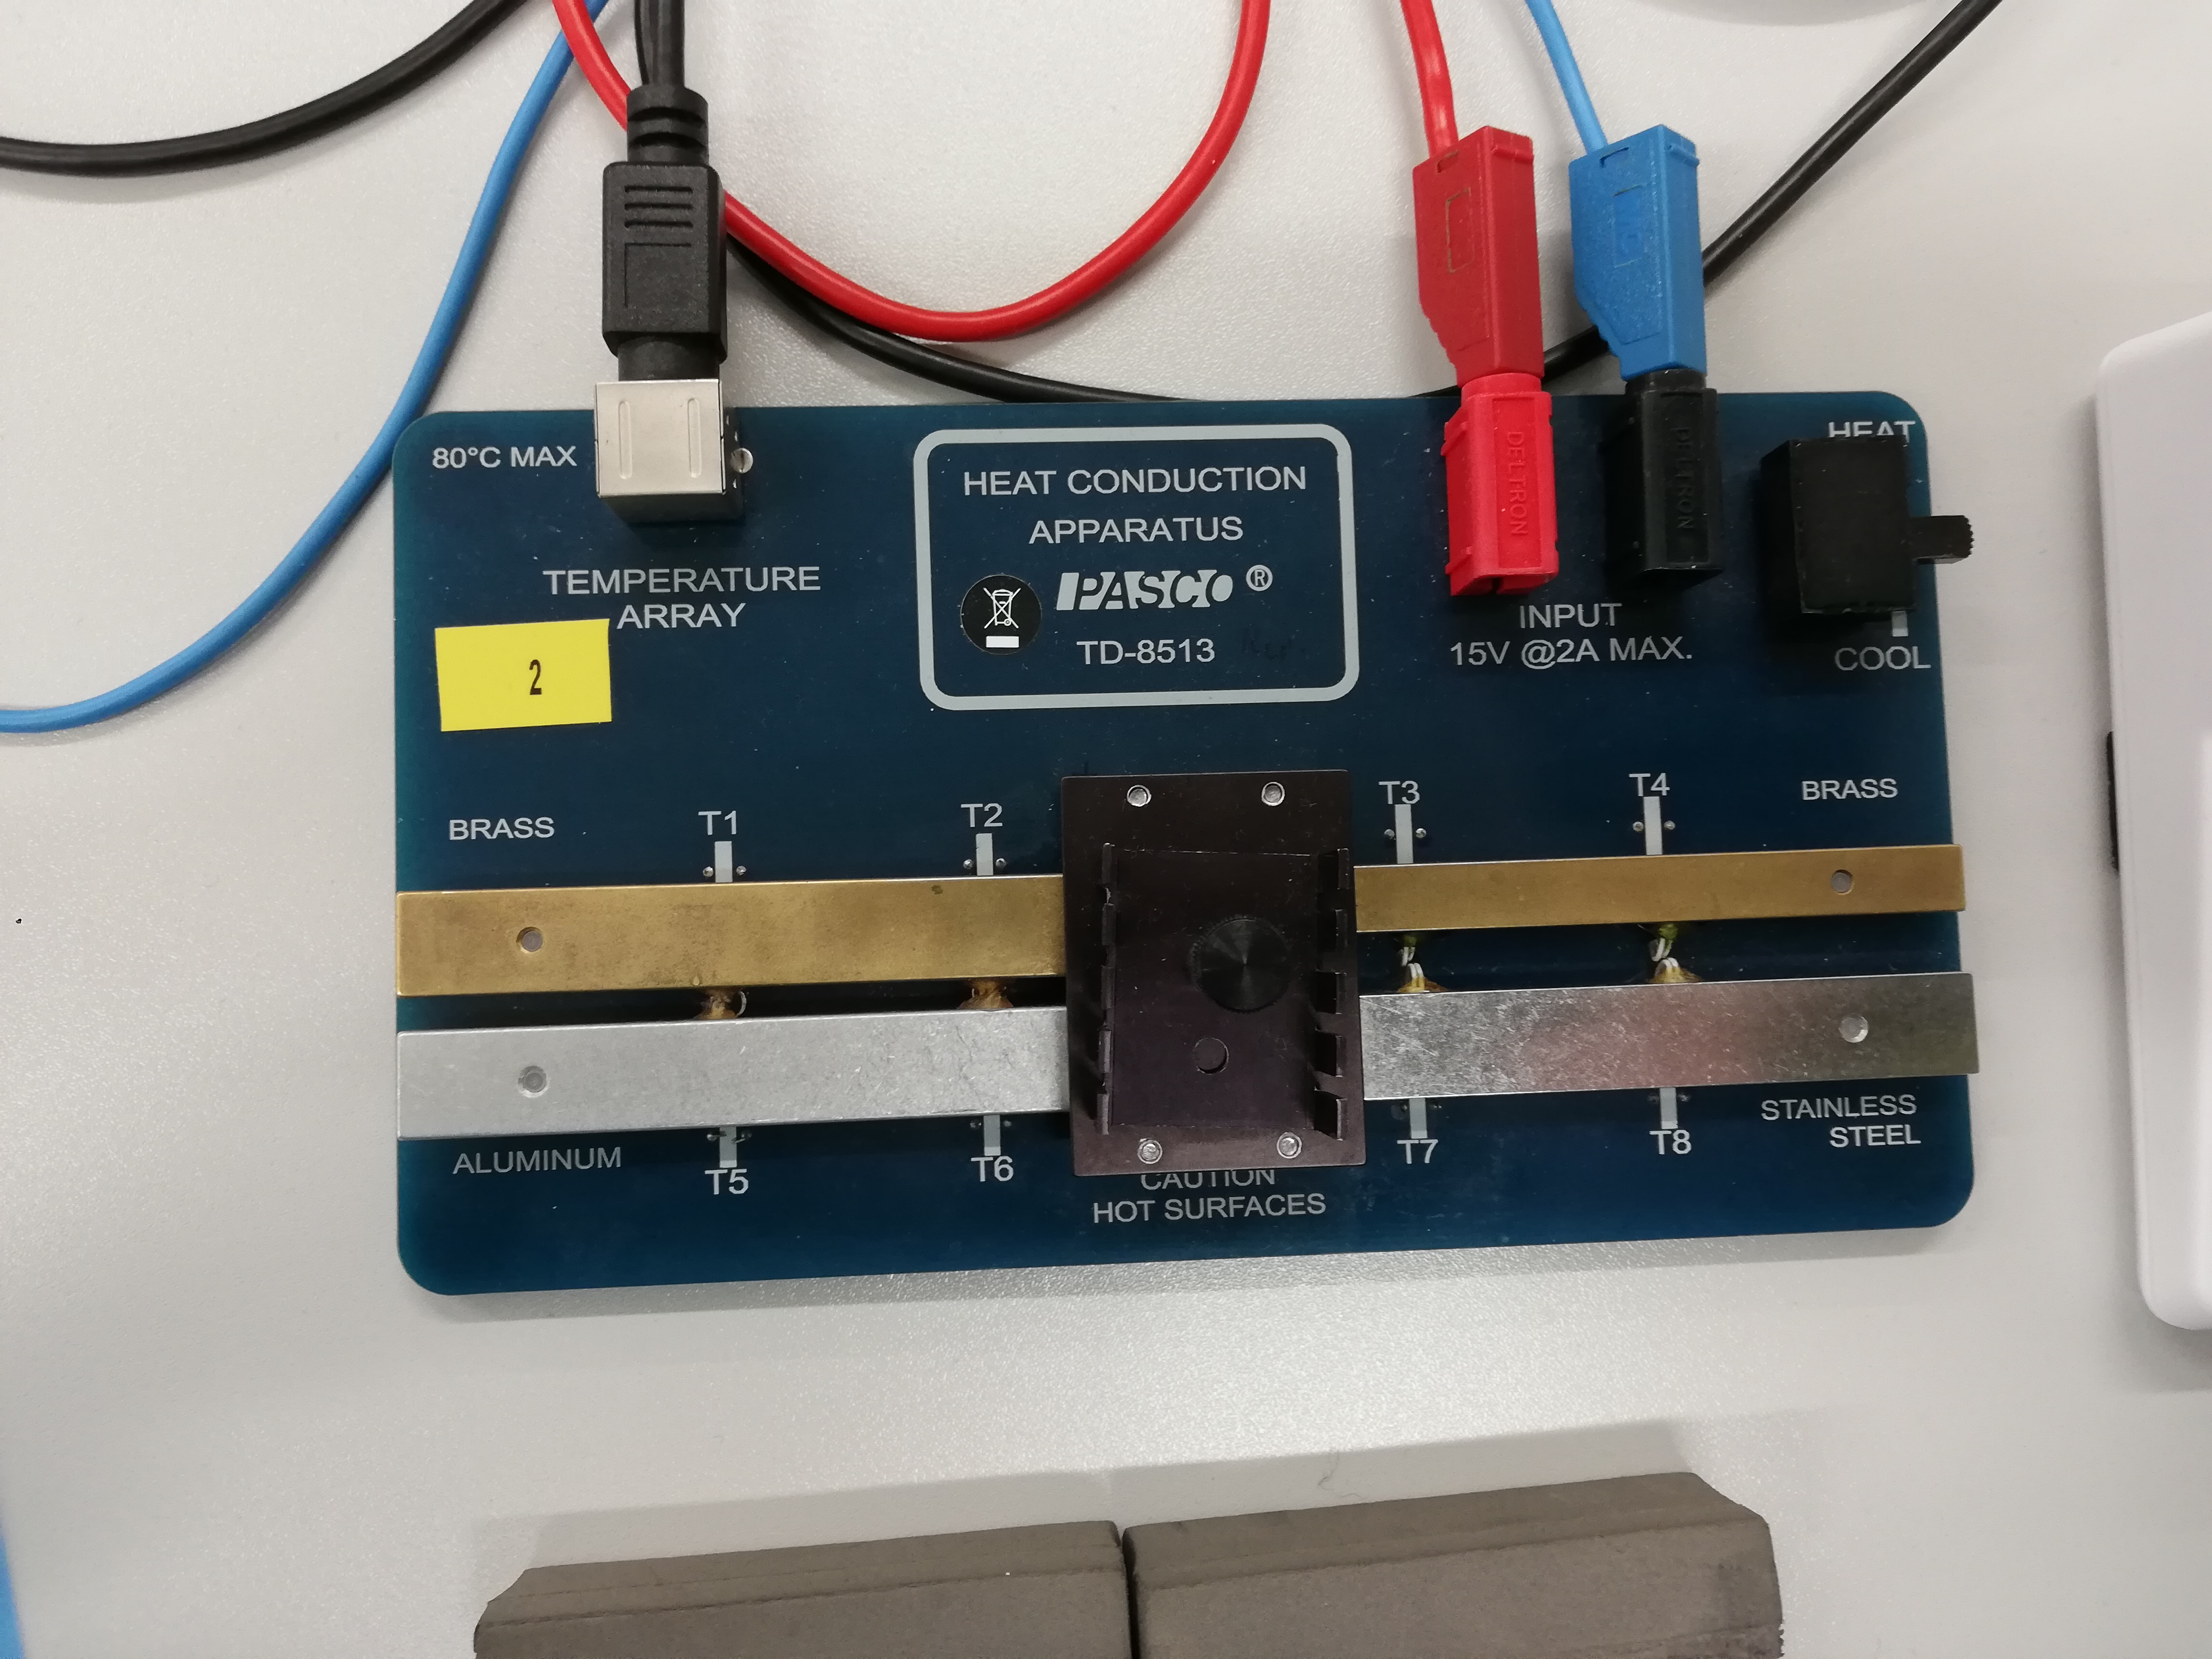
\includegraphics[scale=0.075]{foto_aufbau.jpg}
       \caption{Aufbau der Grundplatte.}
       \label{fig:aufbau}
    \end{figure}

    Die Thermoelemente \textbf{T1} und \textbf{T2} befinden sich am breiten Messingstab,
    die Elemente \textbf{T3} und \textbf{T4} am schmalen Messingstab.
    Am Aluminiumstab befinden sich \textbf{T5} und \textbf{T6}, am Edelstahlstab \textbf{T7} und \textbf{T8}.


    Für die Abmessungen, Dichten, und spezifischen Wärmekapazitäten der Stäbe sind die Werte aus \autoref{tab:vorgegebeneDaten} gegeben.
    \begin{table}
        \centering
        \caption{Eigenschaften der Metallstäbe.}
        \label{tab:vorgegebeneDaten}
        \begin{tabular}{c c c c}
            \toprule
            Material &
            Abmessungen [$\si{\centi\meter}$] &
            $\rho$ [$\si{\kilo\gram\per\cubic\meter}$] &
            $c$ [$\si{\joule\per\kilo\gram\per\kelvin}$] \\
            \midrule
            Messing (breit)   & $9 \times 1.2 \times 0.4$ & 8520 & 385 \\
            Messing (schmal)  & $9 \times 0.7 \times 0.4$ & 8520 & 385 \\
            Aluminium (breit) & $9 \times 1.2 \times 0.4$ & 2800 & 830 \\
            Edelstahl (breit) & $9 \times 1.2 \times 0.4$ & 8000 & 400 \\
            \bottomrule
        \end{tabular}
    \end{table}

    Zur Aufnahme der Messwerte wird ein GLX Datenlogger \enquote{Xplorer GLX} benutzt.
    Dieser wird so eingestellt, dass alle acht Temperaturen der Thermoelemente angezeigt und aufgenommen werden.
    \\
    Während der Messung muss eine Wärmeisolierung über die Stäbe gelegt werden,
    damit möglichst wenig Wärmeaustausch zwischen den Stäben und der Umgebung stattfinden kann.
    Nach jeder Messung werden die Stäbe bis auf eine Temperatur von $\SI{30}{\celsius}$ oder
    weniger gekühlt, bevor eine neue Messung gestartet werden kann.

\subsection{Die statische Methode}

    Bei der statischen Methode wird die Temperatur an den Thermoelementen bei
    laufender Zeit gemessen.
    Zunächchst wird der Abstand $x$ zwischen den Thermoelementen ermittelt.
    Die angelegte Spannung $U_\text{P}$ wird auf $\SI{5}{\volt}$ eingestellt.
    Am Xplorer wird eine Abtastrate $\symup{\Delta} t_\text{GLX} = \SI{5}{\second}$ eingegeben.
    Zum Messen des Temperaturverlaufs wird die Isolierung auf die Stäbe gelegt
    und der Schalter auf \enquote{\textbf{HEAT}} gestellt.
    Die Messung wird solange geführt,
    bis das Thermoelement \textbf{T7} eine Temperatur von ungefähr $\SI{45}{\celsius}$ hat.
    Zudem werden nach $\SI{700}{\second}$ die Temperaturen der Elemente \textbf{T1}, \textbf{T4}, \textbf{T5} und \textbf{T8} aufgeschrieben,
    um zu prüfen, welches Material die beste Leitung besitzt.
    Nach Beenden der Messung werden die Stäbe gekühlt,
    indem der Schalter auf \enquote{\textbf{COOL}} gestellt wird.
    Währenddessen werden die aufgenommenen Messdaten des Xplorers gesichert.
    %Die Wärmeleitfähigkeit soll aus dem Temperaturverlauf berechnet werden.

\subsection{Die dynamische Methode}

    Die dynamische Methode wird auch Angström-Messverfahren genannt.
    Bei dieser Methode werden die Stäbe periodisch erhitzt und gekühlt.
    %Die Wärmeleitfähigkeit kann mithilfe der entstehenden Temperaturwelle berechnet werden.
    Die Spannung $U_\text{P}$ wird bei dieser Methode auf einen Wert von $\SI{8}{\volt}$ eingestellt
    und die Abtastrate des Xplorers auf $\symup{\Delta} t_\text{GLX} = \SI{2}{\second}$.
    Es werden zwei Messungen durchgeführt.\\
    Bei der ersten Messung wird mit einer Periodendauer von $\SI{80}{\second}$ gemessen, wobei
    entsprechend nach $\SI{40}{\second}$ zwischen \enquote{\textbf{HEAT}} und \enquote{\textbf{COOL}} gewechselt wird.
    Es werden mindestens 10 Periodendauern gemessen.
    Anschließend werden die Stäbe wieder gekühlt und die Messdaten gesichert.\\
    Bei der zweiten Messung wird mit einer Periodendauer von $\SI{200}{\second}$ gemessen,
    dementsprechend wird nach $\SI{100}{\second}$ zwischen Kühlen und Erhitzen gewechselt.
    Die Messung wird gestoppt, wenn eines der Thermoelemente \textbf{T1}-\textbf{T8} eine Temperatur von $\SI{80}{\celsius}$
    erreicht hat.
    Nach der Messung werden die Stäbe wieder gekühlt und die Messdaten werden gesichert.
